\section{Vehicle Design}\label{sec:vehicle}%can change title if a better one is found
% Stated in requirements that the vehicle needs to act like a car
% vehicle has four wheels is steered using the front wheels and is driven using the back wheels
% find some sources that give examples of cars looking like what is stated above
% give a description of the car and the fact that it is built using lego

As stated in section \autoref{sec:problem-statement}, one of the requirements for the vehicle is to be similar to an actual car.
The vehicle has been built with four wheels, front wheel steering and is rear wheel driven.
Typically cars have front wheel steering, though more cars have started using four wheel steering.
Rear-wheel drive (RWD) was chosen because it would make the process of building the vehicle smoother, as it would seperate the responsibilities between front and rear wheels.
While there exist all-wheel drive (AWD), front-wheel drive (FWD) and RWD cars, each approach having their own strenghts and weaknesses.
These strengths and weaknesses aren't of vital importance for the project, as the focus is on AVs and automatic driving.
As such, making the process of building the vehicle smoother was prioritized.
\cite{moog_car_steering_2019, collins_car_steering_2018,gareffa_car_drive_2019, glon_car_drive_2019}

To match our choice of hardware, the vehicle will be built using lego.
As we use multiple pieces of hardware from lego, building the vehicle using lego would ensure compatability between the motors, EV3, and the vehicle.
In addition to the lego hardware, we use two other pieces of hardware, namely the Raspberry Pi and the Logitech camera.
In order to ensure both are properly secured to the vehicle, each piece of hardware needs it's own mount.
Additionally, the camera needs to be secured in a way that prevents it from shaking or moving in its mount.
Finally, in order to power the Pi while driving, we need a portable power source.
This portable power source comes in the form of a power bank.

\begin{figure}[H]
    \centering
    \subfloat[Picture from the front of the vehicle]{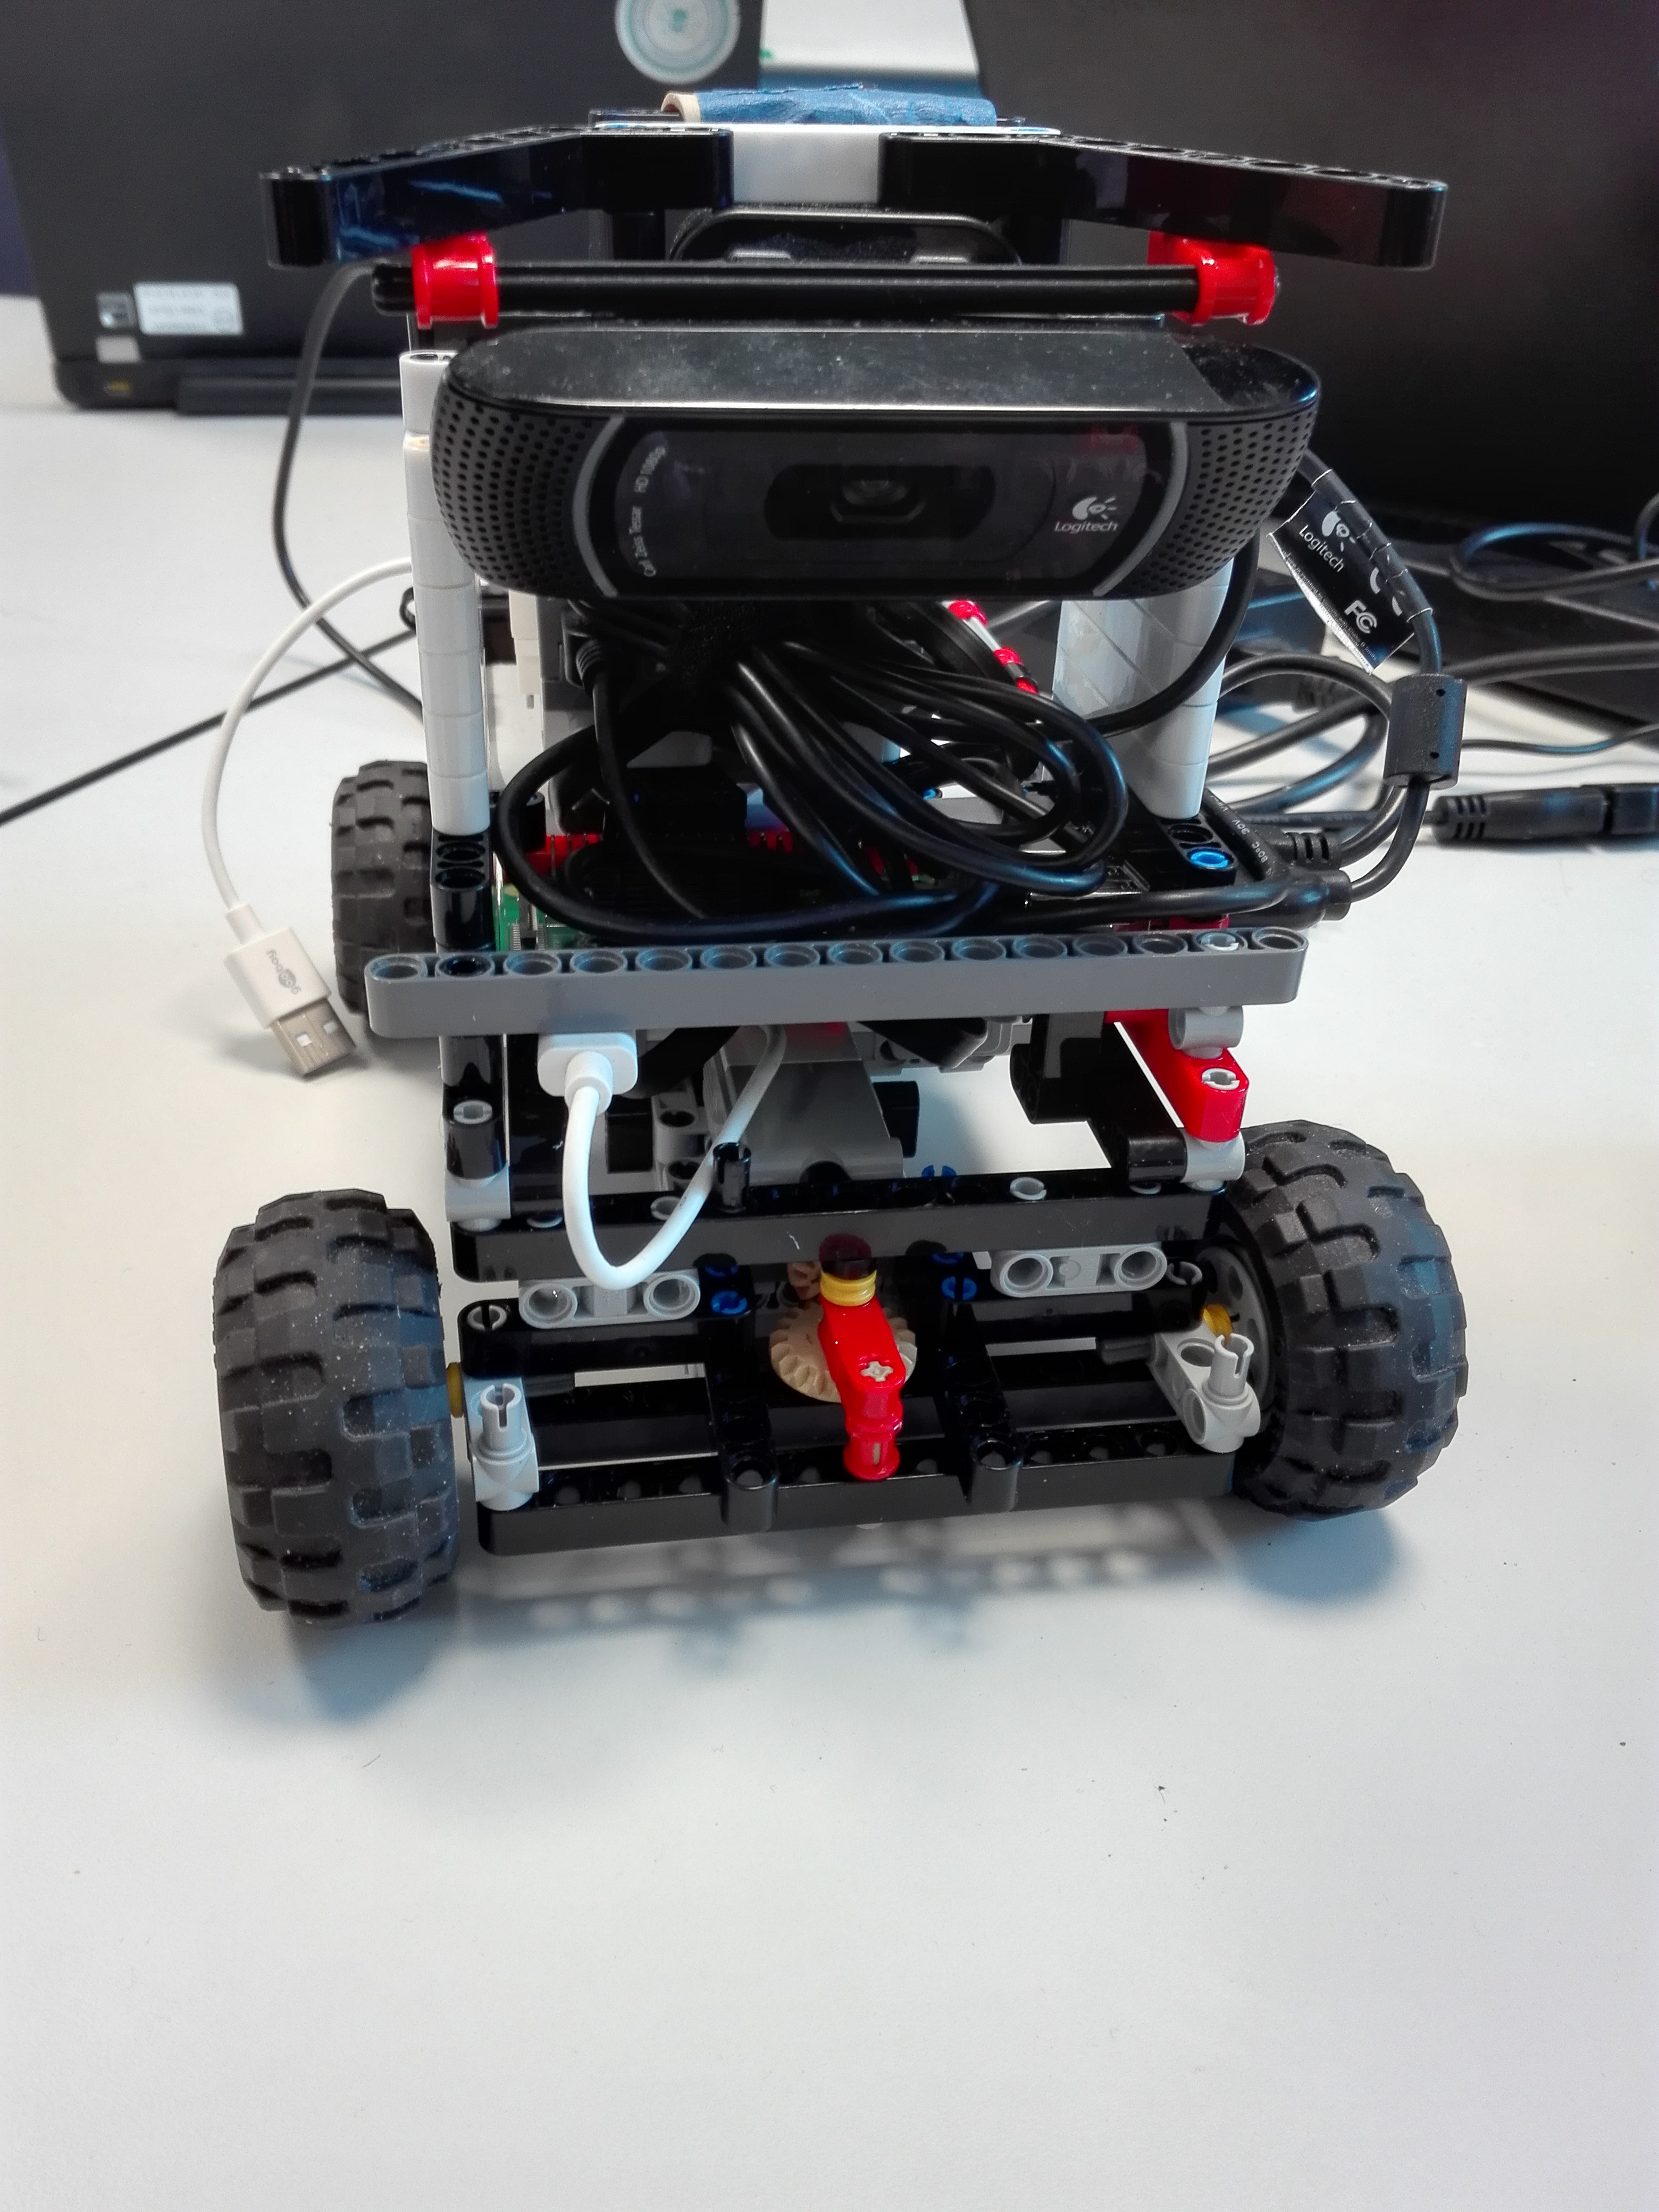
\includegraphics[width=0.5\textwidth]{design/pictureOfVehicle/car_Front.jpg}}
    \subfloat[Picture from the side of the vehicle]{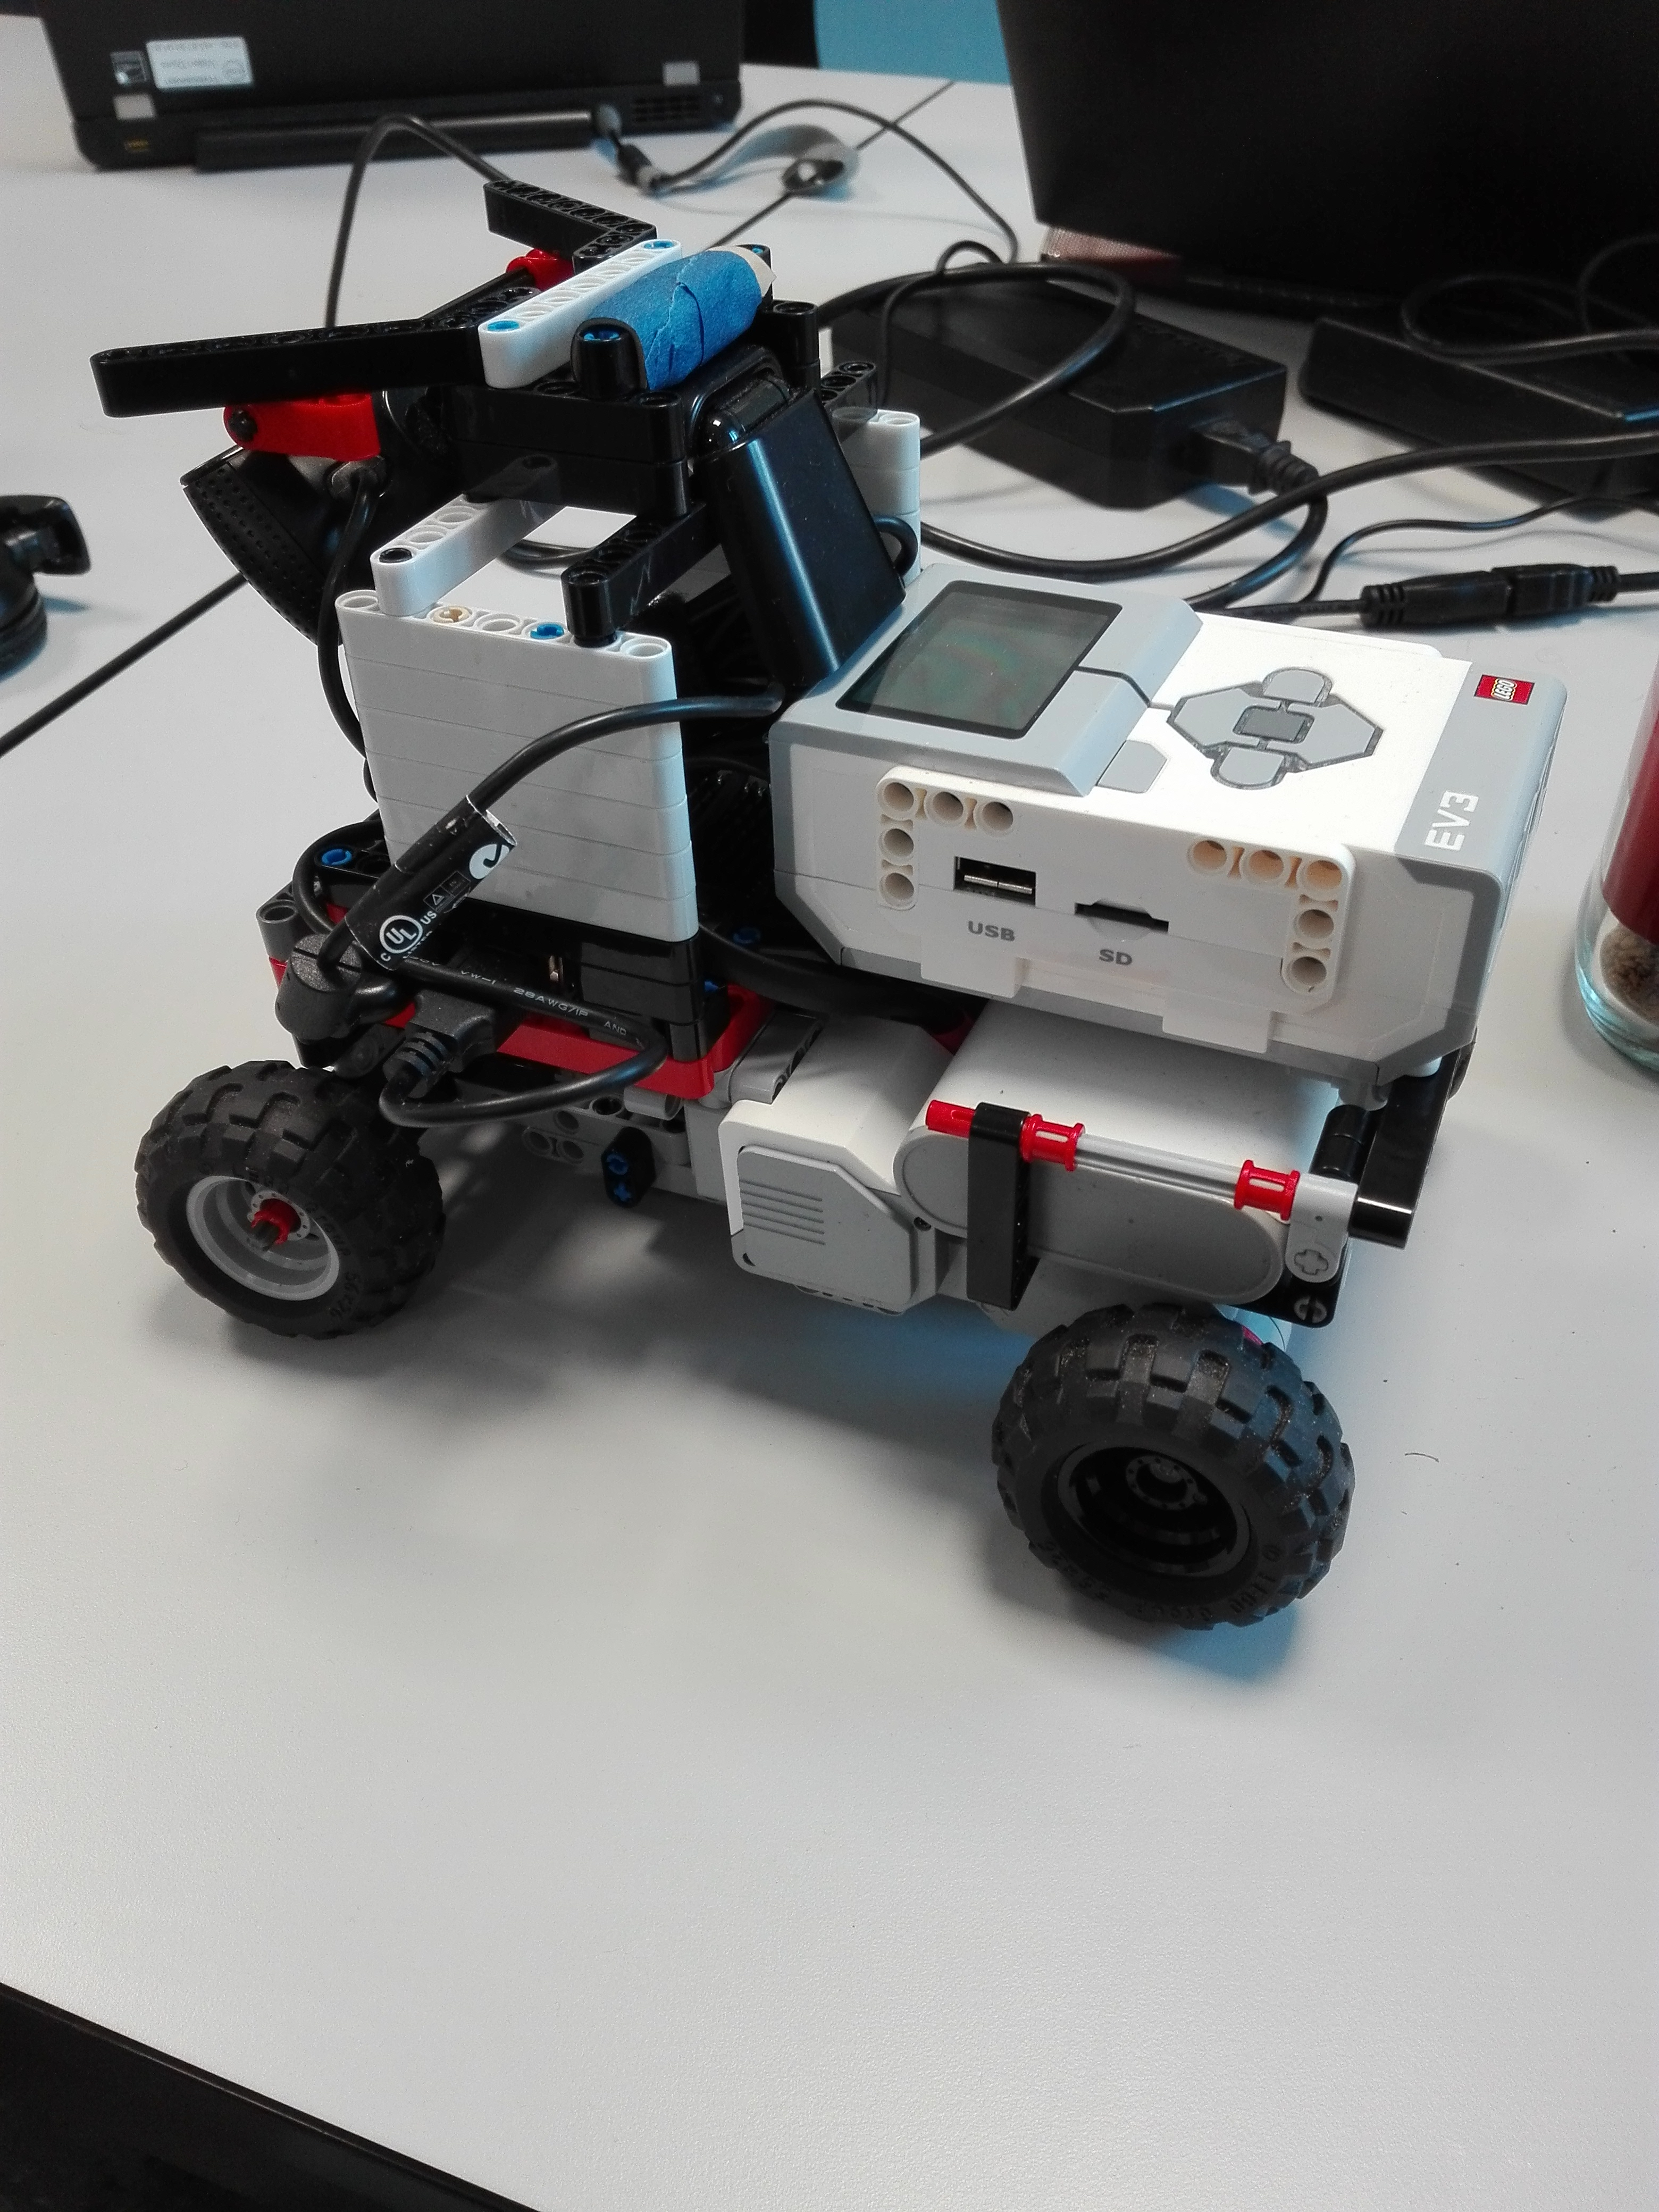
\includegraphics[width=0.5\textwidth]{design/pictureOfVehicle/car_Side.jpg}}
    \caption{Pictures of the finished vehicle taken from different angles}
    \label{fig:design-vehicleDesign-vehicleModel}
\end{figure}

In \autoref{fig:design-vehicleDesign-vehicleModel} are two pictures of the completed vehicle, from the front and side respectivly.
The vehicle has space for all of the components previously described, as well as a functioning mechanism for turning the front wheels.
To allow for the camera to better observe the road, its mount have been built at a higher elevation than the rest of the vehicle.
The mount also uses a rubber band to help secure the camera and prevent it from moving in its mount.
The horizontal "horns" on the mount is to help orient the camera in a consistent manner.
Underneath the camera is a small "case" to secure the raspberry Pi.
This case also allows for the required cables to connect to the Pi.
The EV3 and the powerbank is placed in the of the vehicle.
The EV3 can be connected directly to the vehicle and as such does not need a "case" or mount to secure it to the vehicle.
The powerbank, however, is placed in a small "case" underneath the EV3 where it is secured.
Unfortunately the steering mechanism has a small amount of backlash, which means it is possible to turn the wheels slightly, without affecting the angle of the motor.
This doesn't have an effect on how the software controls the angle of the motor, but it does mean there is an additional inaccuracy when turning the front wheels.
